\lesson{Spotaneity, Entropy, and Gibb's Free Energy}
\subsection{Spontaneous Reactions}
\begin{bulleted-list}
    \item A \textbf{spontaneous} process is one that occurs in a system left to itself. Once started,
        no action from the outside system is necessary to make the process continue
    \item A \textbf{non-spontaneous} process, on the other hand, will not occur unless some external
        action is continuously applied
    \item Example: the rusting of an iron pipe exposed to the atmosphere. Although the process
        occurs quite slowly, it does so continuously. Consequently, the amount of iron decreases
        and the amount of rust increases as time elapses. Therefore, the reaction below is 
        spontaneous
        \[
            \ch{4Fe_{(s)}}+\ch{3O2_{(g)}}\rightleftharpoons \ch{2Fe2O3_{(s)}}
        \]
        The reverse reaction on the other hand is non-spontaneous
\end{bulleted-list}

We can make the following general statements:
\begin{bulleted-list}
    \item If a reaction is \textbf{spontaneous}, then its reverse reaction is \textbf{non-spontaneous}
    \item Both spontaneous and non-spontaneous reactions are possible; however, only the spontaneous
        reaction will occur \textbf{naturally}
    \item Although most exothermic reactions are spontaneous, there are some endothermic reactions
        that are also spontaneous (such as the evaporation of water); therefore, we cannot base
        spontaneity based on enthalpy change
\end{bulleted-list}

\subsection{Entropy - Spontaneity and Disorder}
Consider the analogy in Figure \ref{fig:spontaneity-and-disorder}, where 10 half red half white 
coloured balls are released. If we were to release the balls, which setup would be most likely?
\begin{bulleted-list}
    \item Arrangement (a) is \textbf{not possible}, since the potential energy has not reached
        a minimum
    \item The disorder of (c) makes it more likely than the ordered arrangement in (b)
\end{bulleted-list}
\begin{figure}[ht!]
    \centering
    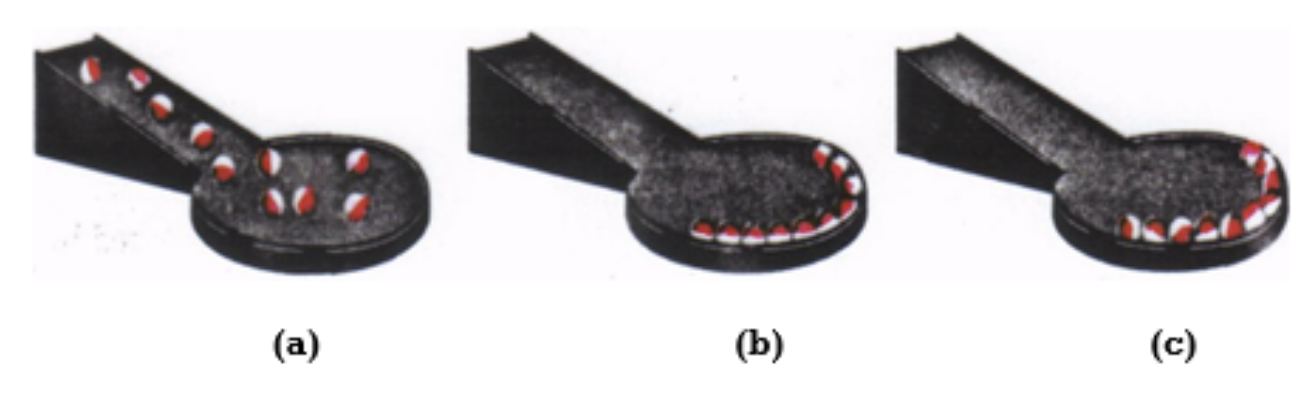
\includegraphics[width=0.6 \textwidth]{../figures/spontaneity-and-disorder.png}
    \caption{}
    \label{fig:spontaneity-and-disorder}
\end{figure}

Consider a situation in which two identical bulbs are filled with ideal gases A and B. Each
bulb has a pressure of 1.00 atm. This is shown in Figure \ref{fig:ideal-gases-spontaneity-and-disorder}
\begin{bulleted-list}
    \item A stopcock valve joins the two bulbs. When the valve is opened, assuming the two gases
        do not react, then each gas is going to expand into the bulb, containing the other gas
        and will continue mixing until the partial pressure of each gas is 0.500 atm in each bulb
\end{bulleted-list}

\begin{figure}[ht!]
    \centering
    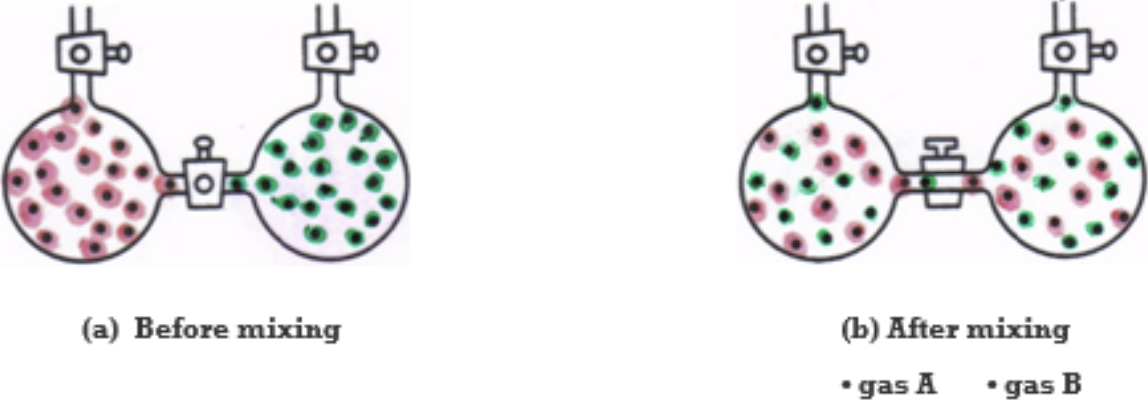
\includegraphics[width=0.6 \textwidth]{../figures/ideal-gases-spontaneity-and-disorder.png}
    \caption{}
    \label{fig:ideal-gases-spontaneity-and-disorder}
\end{figure}

\begin{important}
    One of the characteristics of an ideal gas is that its interal energy ($E$) and enthalpy
    ($H$) depend only on temperature and NOT on pressure or volume. Recall there are no IMF 
    between gases A and B, when these two ideal gases mix at a constant temperature, 
    $\Delta E=PV+\Delta H\approx\Delta H=0$, recalling that $PV\approx 0$. Therefore, enthalpy
    is NOT the driving force behind the spontaneous mixing of gases. The driving force is simply
    the tendency of molecules to arrange themselves in the most random or \textbf{disordered} manner.
\end{important}

What is \textbf{entropy}?
\begin{bulleted-list}
    \item \textbf{Entropy}, denoted by $S$, is the thermodynamic property related to the
        degree of disorder in a system. The greater the degree of randomness or disorder in a system
        the greater its entropy
    \item Like internal energy and enthalpy, etropy is a \textit{function of state}. Entropy has
        a unique value for a system whose temperature, pressure, and composition are specified
    \item The \textbf{entropy change}, $\Delta S$, is the difference in entropy between two states
        and also has a unique value
    \item The formula for standard entropy change is
        \[
            \Delta S^{\circ}=\Sigma n_pS^{\circ}_\text{products}-\Sigma n_fS^{\circ}_\text{reactants}
        \]
\end{bulleted-list}

In general, a system will experience an increase in entropy ($\Delta S>0$) if:
\begin{bulleted-list}
    \item The volume of the gaseous system increases
    \item The temperature of the system increases
    \item The physical state of a system changes from solid to liquid or gas, or liquid to gas
        ($\S_\mathrm{gas}>S_\mathrm{liquid}>S_\mathrm{solid}$)
\end{bulleted-list}

In chemical reactions, entropy increases ($\Delta S>0$) when:
\begin{bulleted-list}
    \item Fewer moles of reactant molecules form a greater number of moles of product molecules.
        For instance, the reverse reaction of the Haber process
        \[
            \ch{2NH3_{(g)}}\rightleftharpoons \ch{N2_{(g)}}+\ch{3H2_{(g)}}
        \]
    \item Complex molecules are broken down into simpler subunits
        \[
            \ch{C6H12O6_{(s)}}+\ch{6O2_{(g)}}\rightleftharpoons \ch{6CO2_{(g)}}+\ch{6H2O_{(g)}}
        \]
    \item Solid reactants become liquid or gaseous products (or liquids become gases)
        \[
            \ch{2H2O_{(\ell)}}\rightleftharpoons \ch{2H2_{(g)}}+\ch{O2_{(g)}}
        \]
\end{bulleted-list}

\begin{figure}[ht!]
    \centering
    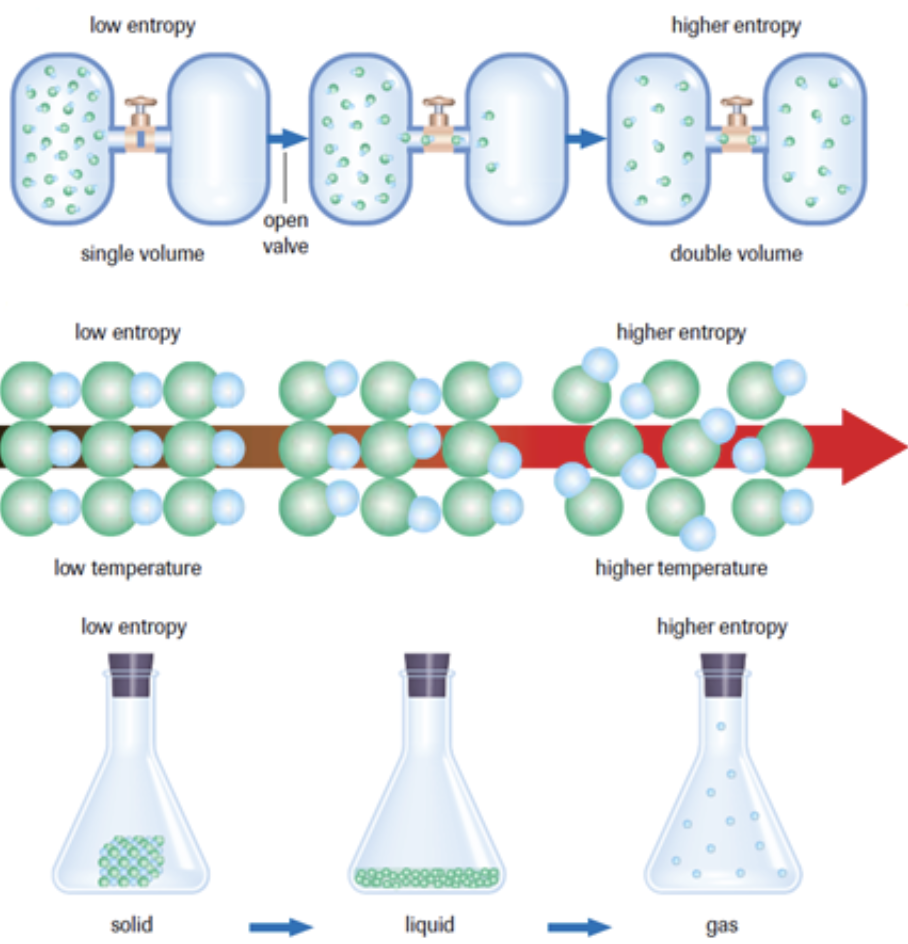
\includegraphics[width=0.8 \textwidth]{../figures/entropy.png}
\end{figure}

\subsection{Free Energy}
\begin{bulleted-list}
    \item Gibbs concluded that the spontaneity of a reaction depends on both enthalpy and
        entropy
    \item Gibbs Free Energy is the energy available to do work and is calculated as
        \[
            G=H-TS
        \]
    \item The free energy change is
        \[
            \Delta G=\Delta H-T\Delta S
        \]
    \item When $\Delta G<0$, the reaction is \textbf{spontaneous}
    \item When $\Delta G>0$, the reaction is \textbf{non-spontaneous}
    \item When $\Delta G=0$, the reaction is at equilibrium
\end{bulleted-list}

\begin{important}
    Note that the entropy change is measured in units \si{J.mol^{-1}.K^{-1}}, while enthalpy is
    measured in units \si{kJ.mol^{-1}}. Keep an eye out for joules vs kilojoules.
\end{important}

\begin{table}[!ht]
    \centering
    \caption{We can use the end behaviour with respect to temperature, T}
    \setlength{\tabcolsep}{12pt}      % column spacing
    \renewcommand{\arraystretch}{1.2} % row spacing
    \arrayrulecolor{black}            % table border color
    \begin{tabular}{|c|c|c|c|}
        \hline
        \rowcolor{HeaderColor}
        $\Delta G$ & $\Delta H$ & $\Delta S$ & $\Delta G=\Delta H-T\Delta S$ \\ \hline
        always spontaneous & negative & positive & negative at all temperatures \\ \hline
        spontaneous at high temperatures & positive & positive & negative at high temperatures \\ \hline
        spontaneous at low temperatures & negative & negative & negative at low temperatures \\ \hline
        always non-spontaneous & positive & negative & positive at all temperatures \\ \hline
    \end{tabular}
\end{table}

For instance, in an exothermic reaction, we can calculate the Gibbs free energy to determine the
spontaneity of the reaction. In an exothermic reaction, $\Delta H<0$, due to it releasing energy.
Furthermore, $\Delta S>0$, since the entropy of the system is greater by either forming more
moles of product or forming all gas products. Therefore, $\Delta G<0$ no matter what temperature,
hence an exothermic reaction is spontaneous.

\begin{figure}[ht!]
    \centering
    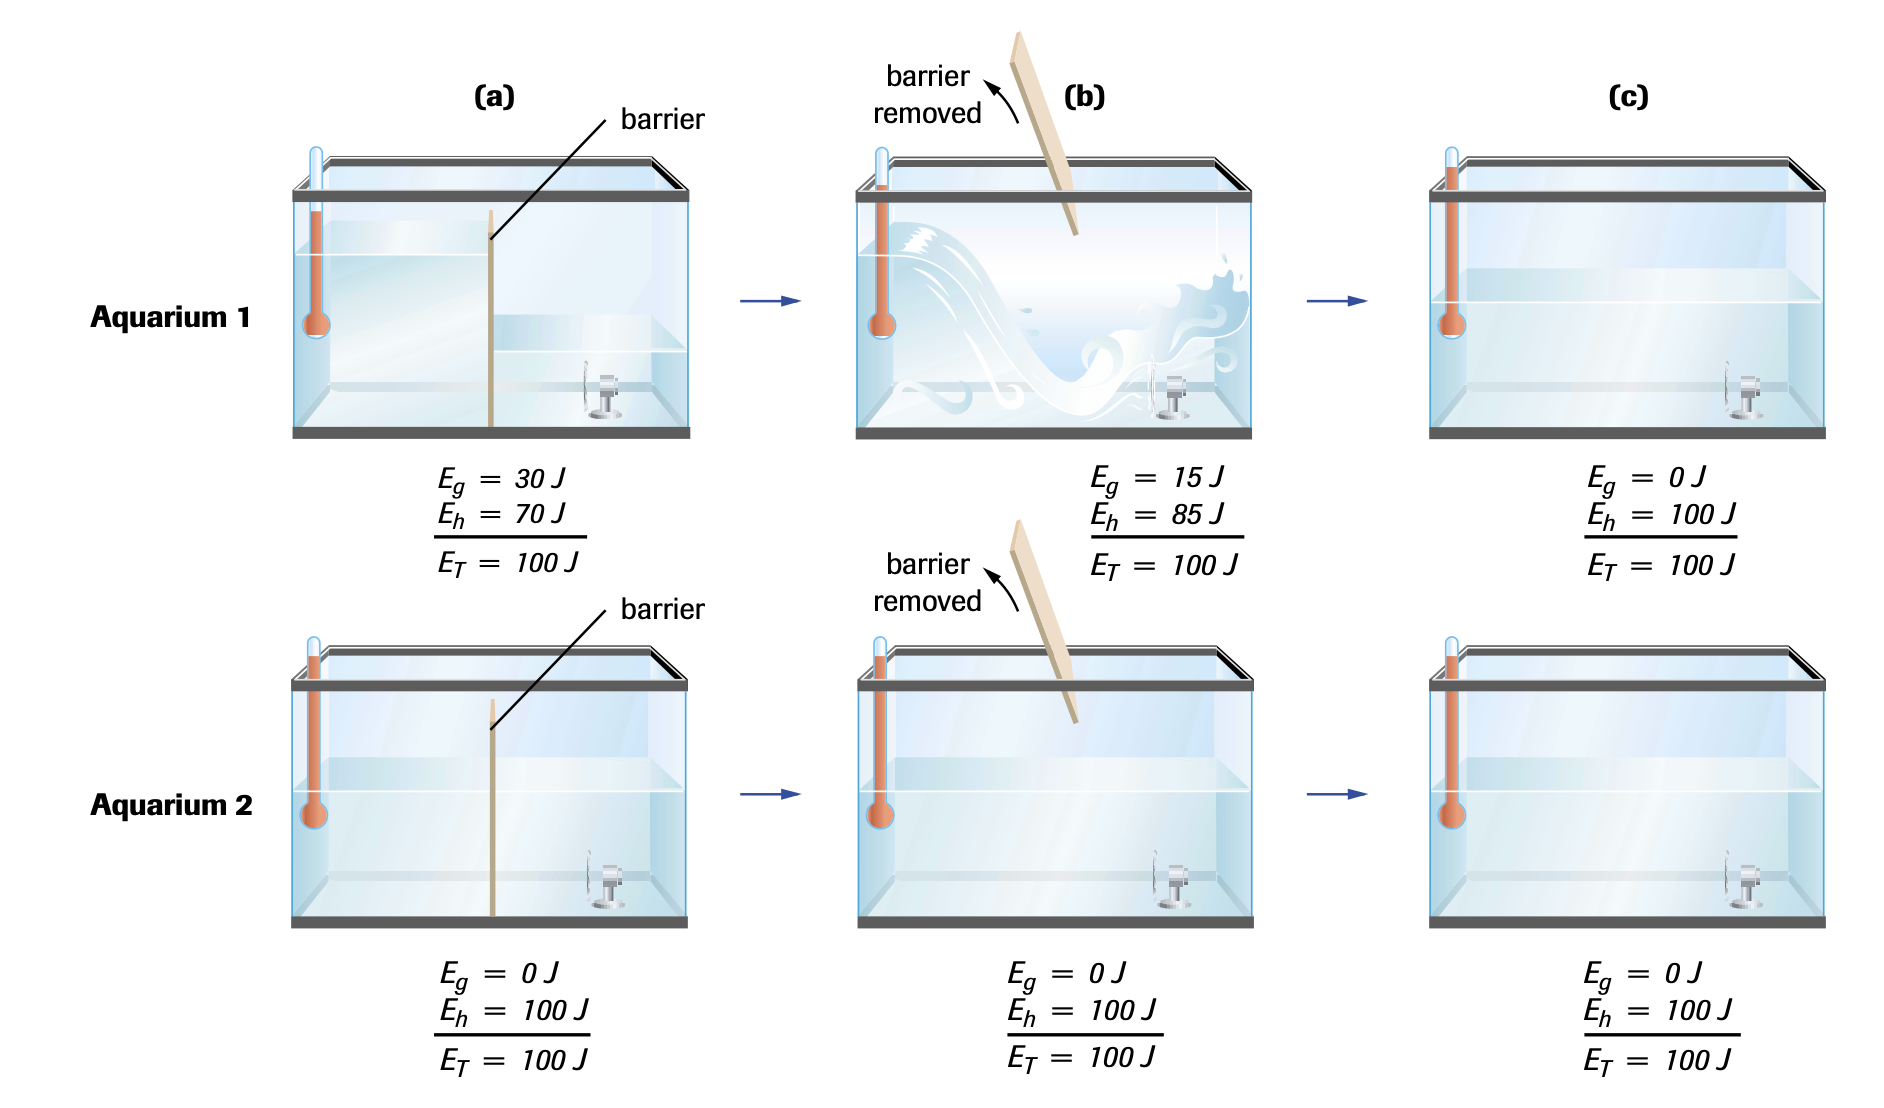
\includegraphics[width=0.8 \textwidth]{../figures/aquarium-analogy.png}
    \caption{In (a), $G>0$ and $\Delta G=0$ (ordered); the reaction is non-spontaneous, external 
        action needs to be applied for the process to occur. In (b), $G>0$ and $\Delta G<0$ 
        (disordered); the reaction is spontaneous, no external action needs to be applied for
        the process to occur. In (c), $G=0$ and $\Delta G=0$ (equilibrium).}
    \label{fig:aquarium-analogy}
\end{figure}

\subsection{First Law of Thermodynamics}
The total amount of energy in the universe is constant. Energy can be neither created nor destroyed,
but can be transferred from one object to another, or transformed from one form to another.

\subsection{Second Law of Thermodynamics}
All changes either directly or indirectly increase the entropy of the universe. Mathematically
\[
    \Delta S_\mathrm{universe}>0
\]

\subsection{Third Law of Thermodynamics}
The entropy of a perfectly ordered pure crystalline substance is 0 at absolute zero. Mathematically
\[
    S=0\quad\text{at}\quad T=0\,\si{K}
\]

\subsection{Equilibrium and $\Delta G$}
Consider Figure \ref{fig:battery}. When fully charged, the unequal distribution of charge on two
sides of an insulator is maximal and the value of $\Delta G$ for the system is large and negative.
When a conductor is connected betwene the two terminals, charges \textbf{spontaneously} flow from
the negative terminal to the positive terminal, generating current and hence voltage. However,
this flow increases the value of $\Delta G$ and releases free energy that is able to perform
useful work, in this case lighting the lightbulb. When the electrical charges become equally
distributed between the two compartments, dynamic equilibrium is achieved and the value of
$\Delta G=0$. No net movement of charge is possible, and no more work can be extracted from
the system. 

\begin{figure}[ht!]
    \centering
    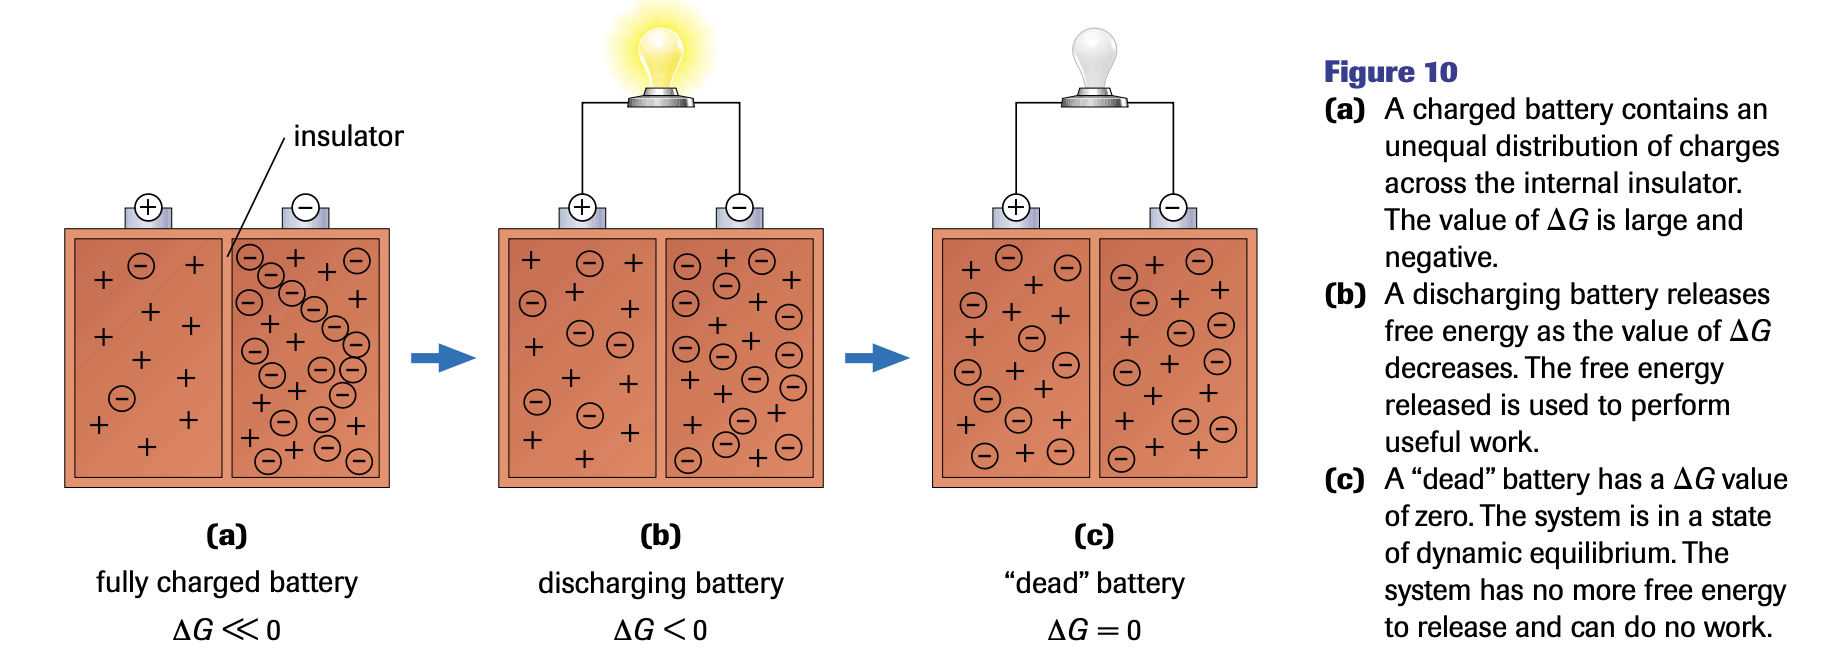
\includegraphics[width=\textwidth]{../figures/battery}
    \caption{}
    \label{fig:battery}
\end{figure}

For instance, consider liquid water being cooled to a temperature below its freezing point at
101.3 kPa of pressure
\[
    \ch{H2O_{(\ell)}}\rightleftharpoons \ch{H2O_{(s)}}
\]
Above $0^{\circ}$C, $\Delta G>0$ and freezing is nonspontaneous ($\Delta H\leq0$ and $\Delta S<0$),
thus the water remains liquid. At exactly $0^{\circ}$C, the system is in a state of dynamic
equilibrium as an ice-water mixture: slush. The water remains as slush as long as the temperature
is $0^{\circ}$C, and the water becomes ice once the temperature is below $0^{\circ}$C ($\Delta G<0$)
